\begin{figure}[h]
		\begin{center}
			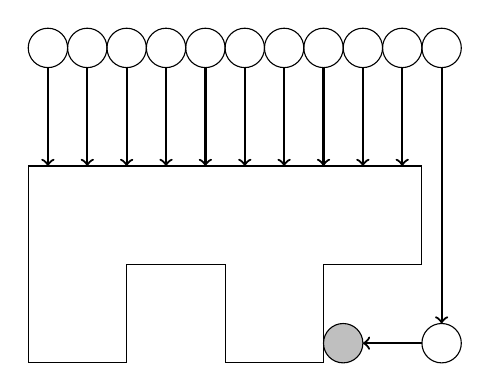
\begin{tikzpicture}
				\draw (0, 0)--(5, 0);
				\draw (5, 0)--(5, -1.25);
				\draw (5, -1.25)--(3.75, -1.25);
				\draw (3.75, -1.25)--(3.75, -2.5);
				\draw (3.75, -2.5)--(2.5, -2.5);
				\draw (2.5, -2.5)--(2.5, -1.25);
				\draw (2.5, -1.25)--(1.25, -1.25);
				\draw (1.25, -1.25)--(1.25, -2.5);
				\draw (1.25, -2.5)--(0, -2.5);
				\draw (0, -2.5)--(0,0);
				
				\draw (0.25, 1.5) circle (0.25);
				\draw (0.75, 1.5) circle (0.25);
				\draw (1.25, 1.5) circle (0.25);
				\draw (1.75, 1.5) circle (0.25);
				\draw (2.25, 1.5) circle (0.25);
				\draw (2.75, 1.5) circle (0.25);
				\draw (3.25, 1.5) circle (0.25);
				\draw (3.75, 1.5) circle (0.25);
				\draw (4.25, 1.5) circle (0.25);
				\draw (4.75, 1.5) circle (0.25);
				\draw (5.25, 1.5) circle (0.25);
				\draw (5.25, -2.25) circle (0.25);
				\draw (4, -2.25)[fill=gray!50] circle (0.25);
				
				\draw[->, thick] (0.25, 1.25) -- (0.25, 0);
				\draw[->, thick] (0.75, 1.25) -- (0.75, 0);
				\draw[->, thick] (1.25, 1.25) -- (1.25, 0);
				\draw[->, thick] (1.75, 1.25) -- (1.75, 0);
				\draw[->, thick] (2.25, 1.25) -- (2.25, 0);
				\draw[->, thick] (2.75, 1.25) -- (2.75, 0);
				\draw[->, thick] (3.25, 1.25) -- (3.25, 0);
				\draw[->, thick] (3.75, 1.25) -- (3.75, 0);
				\draw[->, thick] (4.25, 1.25) -- (4.25, 0);
				\draw[->, thick] (4.75, 1.25) -- (4.75, 0);
				\draw[->, thick] (5.25, 1.25) -- (5.25, -2);
				\draw[->, thick] (5, -2.25) -- (4.25, -2.25);
			\end{tikzpicture}
		\end{center}
		\caption{Расположение второй фигуры <<тетрисным>> способом}
		\label{second_tetris}
	\end{figure}